\section{An overview of the data}

\frame{\frametitle{Structure}
    A large corpus of patient-episode data has been provided by the Cwm Taf
    University Health Board over the period April 2013 through April 2017. The
    data has the following structure for individual patients:

    \begin{table}[htbp]
        \resizebox{.9\textwidth}{!}{%
            \begin{tabular}{lllrrlllr}
\toprule
&            &              &      Net Cost &   Age (years) &    HRG &
Admission Date &    Discharge Date &  Length of Stay (days) \\
PATIENT ID & SPELL ID & EPISODE ID &              &       &        &             &             &           \\
\midrule
ID\_123456 & M1001 & M1001-1 &   858.14 &  74 &  EA05Z &  2015-05-06 &  2015-05-06 &       0.0 \\
                   & M1211 & M1211-1 &   333.95 &  74 &  FZ38F &  2015-07-15 &  2015-08-01 &      17.0 \\
                   &            & M1211-2 &   706.09 &  74 &  FZ38F &  2015-07-15 &  2015-08-01 &      17.0 \\
                   &            & M1211-3 &  8671.31 &  74 &  RC16Z &  2015-07-15 &  2015-08-01 &      17.0 \\
\bottomrule
\end{tabular}

        }
    \end{table}

    \pause%
    Each episode (row) has a number of associated measurements (columns),
    including:
    \begin{itemize}
        \pause\item personal and demographic identifiers;
        \pause\item condition and procedure codes;
        \pause\item other clinical references;
        \pause\item cost components
    \end{itemize}
}

\subsection{Distributions of key attributes}

\frame{\frametitle{Number of spells associated with a patient}
    \centering
    \includegraphics[width=\imgwidth]{no_spells_hist/main.pdf}
}

\frame{\frametitle{Length of stay}
    \centering
    \includegraphics[width=\imgwidth]{los_hist/main.pdf}
}

\frame{\frametitle{Net cost of a spell}
    \centering
    \includegraphics[width=\imgwidth]{netcost_kde/main.pdf}
}

\frame{\frametitle{Number of diagnoses in an episode}
    \centering
    \includegraphics[width=\imgwidth]{no_diag_hist/main.pdf}
}

\frame{\frametitle{Number of procedures in an episode}
    \centering
    \includegraphics[width=\imgwidth]{no_proc_hist/main.pdf}
}

\subsection{Demographic information}

\frame{\frametitle{Demographic information}
    There are issues with demographic information in the data:

    \begin{itemize}
        \pause\item Gender is binary and inconsistently recorded
    \pause\item Limited geographic information encoded in registered GP
        practice
    \end{itemize}
}

\frame{\frametitle{Distribution of age}
    \centering
    \includegraphics[width=\imgwidth]{age_hist/main.pdf}
}

\subsection{Correlation and interaction}

\frame{\frametitle{Pairwise correlation}
    \centering
    \includegraphics[width=\imgwidth]{corr_heatmap/main.pdf}
}

\frame{\frametitle{Detecting collinearity}

    \centering
    \begin{minipage}{.8\imgwidth}
        \resizebox{\linewidth}{!}{%
            \begin{tabular}{lrrrrrrrrrr}
\toprule
Attribute &  Intercept &  CRIT &     DRUG &    EMER &    ENDO &     HCD &     IMG &  IMG\_OTH &      MED &     NCI \\
\midrule
Coefficient               &     1737.6 &   0.3 &    315.7 &    29.2 &    93.0 &   215.8 &   141.7 &      1.4 &    738.2 &    85.1 \\
t-Value                   &    68692.0 &   8.3 &  10666.0 &  1151.6 &  3570.7 &  8332.6 &  3036.9 &     29.8 &  16631.1 &  2297.4 \\
p-Value                   &        0.0 &   0.0 &      0.0 &     0.0 &     0.0 &     0.0 &     0.0 &      0.0 &      0.0 &     0.0 \\
Variance Inflation Factor &        NaN &   1.6 &      1.4 &     1.0 &     1.1 &     1.0 &     3.4 &      3.3 &      3.1 &     2.1 \\
\bottomrule
\end{tabular}

    }
    \end{minipage}

    \begin{minipage}{.8\imgwidth}
        \resizebox{\linewidth}{!}{%
            \begin{tabular}{lllllllllll}
\toprule
Attribute &      NID &    OCLST &     OPTH &     OTH & OTH\_OTH &     OUTP &      OVH &    PATH & PATH\_OTH &     PHAR \\
\midrule
Coefficient               &   242.04 &       60 &   478.71 &   13.96 &   -1.53 &    27.02 &    735.4 &  142.72 &    -5.03 &    86.45 \\
t-Value                   &  5820.74 &  2124.75 &  13739.1 &  268.32 &  -29.47 &  1058.65 &  9654.74 &  2097.3 &   -79.39 &  2316.56 \\
p-Value                   &     0.00 &     0.00 &     0.00 &    0.00 &    0.00 &     0.00 &     0.00 &    0.00 &     0.00 &     0.00 \\
Variance Inflation Factor &      2.7 &     1.25 &      1.9 &    4.23 &    4.21 &     1.02 &     9.07 &    7.24 &     6.27 &     2.18 \\
\bottomrule
\end{tabular}

        }
    \end{minipage}

    \begin{minipage}{.8\imgwidth}
        \resizebox{\linewidth}{!}{%
            \begin{tabular}{llllllllll}
\toprule
Attribute &    PROS &   RADTH &     SECC &      SPS &     THER &     WARD & TRUE\_LOS & DIAG\_NO & PROC\_NO \\
\midrule
Coefficient               &  342.92 &    7.95 &     27.3 &   149.17 &   181.56 &  1226.31 &    -1.74 &    0.51 &       1 \\
t-Value                   &   13241 &  310.74 &  1076.82 &  5827.14 &  6365.45 &  21362.3 &   -30.18 &    18.2 &   34.09 \\
p-Value                   &    0.00 &    0.00 &     0.00 &     0.00 &     0.00 &     0.00 &     0.00 &    0.00 &    0.00 \\
Variance Inflation Factor &    1.05 &    1.02 &        1 &     1.02 &     1.27 &     5.15 &     5.17 &    1.24 &    1.34 \\
\bottomrule
\end{tabular}

        }
    \end{minipage}

    \begin{minipage}{.8\imgwidth}
        \resizebox{\linewidth}{!}{%
            \begin{tabular}{lrrrrrrr}
\toprule
Attribute &  RADTH &    SECC &     SPS &    THER &     WARD &  TRUE\_LOS &  DIAG\_NO \\
\midrule
Coefficient               &    7.9 &    27.3 &   149.1 &   182.0 &   1234.8 &      -1.1 &      0.5 \\
t-Value                   &  307.8 &  1066.5 &  5775.0 &  6338.1 &  21620.2 &     -21.6 &     17.9 \\
p-Value                   &    0.0 &     0.0 &     0.0 &     0.0 &      0.0 &       0.0 &      0.0 \\
Variance Inflation Factor &    1.0 &     1.0 &     1.0 &     1.3 &      5.0 &       3.7 &      1.2 \\
\bottomrule
\end{tabular}

        }
    \end{minipage}
}

\subsection{Measuring variation and relative importance}

\frame{\frametitle{Cost variation}
    \centering
    \includegraphics[width=\imgwidth]{cost_variation/main.pdf}
}

\frame{\frametitle{Component contribution to net costs}
    \centering
    \includegraphics[width=\imgwidth]{cost_contribution/main.pdf}
}

\frame{\frametitle{Relative importance}
    \centering
    \includegraphics[width=\imgwidth]{cost_bubble_plot/main.pdf}
}
